\part{Application Domain Analysis}
\begin{figure}[H]
    \begin{tabular}{|l|p{12cm}|}
        \hline
        \textbf{Purpose} & \begin{itemize}
            \item To determine a system's usage requirements.
        \end{itemize} \\\hline
        \textbf{Concepts} & \begin{itemize}
            \item Application domain: An organizarion that administrates, monitors, or controls a problem domain.
            \item Requirements: A system's externally observable behavior.
        \end{itemize} \\\hline
        \textbf{Principles} & \begin{itemize}
            \item Determine the application domain use cases.
            \item Collaborate with users.
        \end{itemize} \\\hline
        \textbf{Result} & \begin{itemize}
            \item A completelist of the system's overall usage requirements.
        \end{itemize} \\\hline
    \end{tabular}
\end{figure}
Concepts:
\begin{itemize}
    \item Actors (Users and other systems)
    \item Use cases
    \item Functions
    \item Interfaces
\end{itemize}
\begin{figure}[]
    \centering
    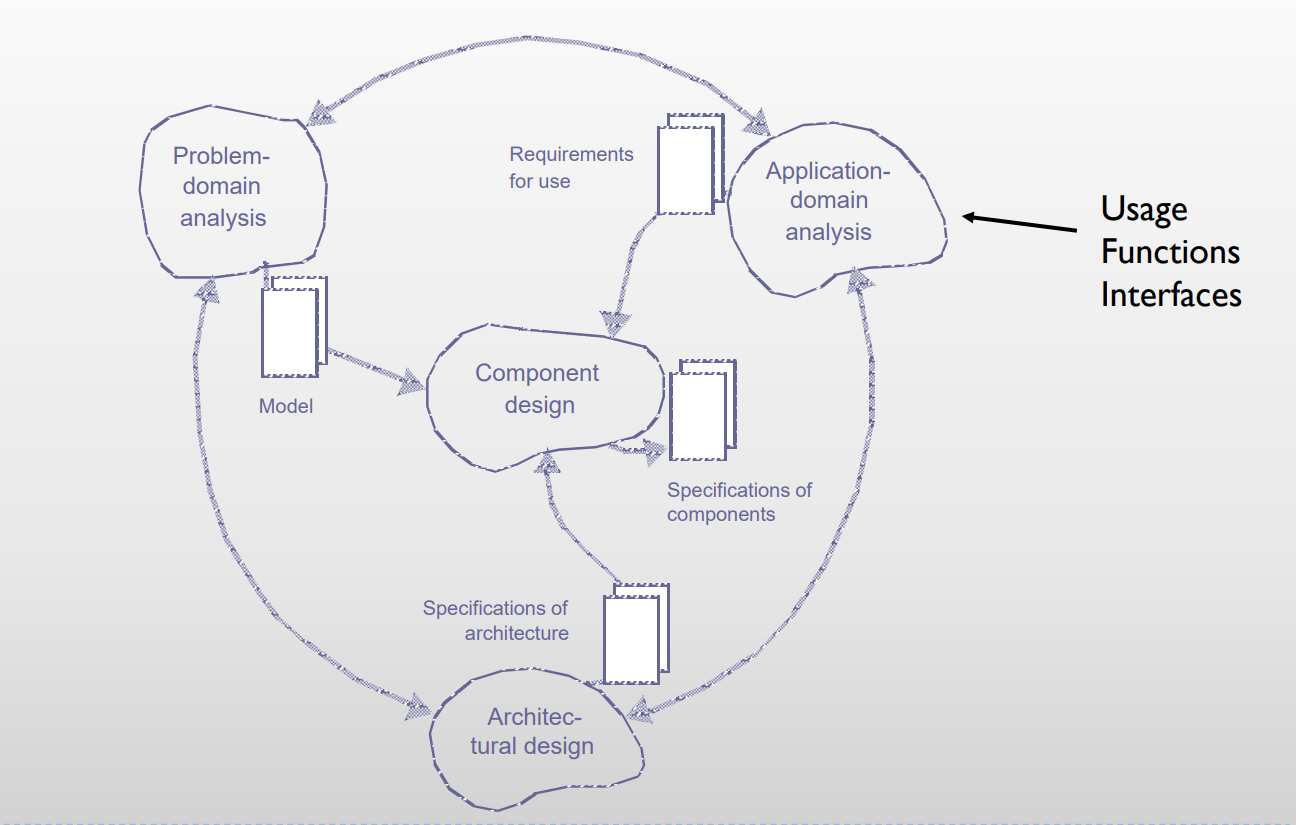
\includegraphics[width=\linewidth]{parts/3_application_domain_analysis/figures/activities.png}
    \caption{Application Domain Analysis: Activities}
\end{figure}
\chapter{Usage \ooad[121]}
\begin{figure}[H]
    \begin{tabular}{|l|p{12cm}|}
        \hline
        \textbf{Purpose} & \begin{itemize}
            \item To determine how actors interact with a system.
        \end{itemize} \\\hline
        \textbf{Concepts} & \begin{itemize}
            \item Actor: An abstraction of users or other systems that interact with the target system.
            \item Use case: A pattern for interaction between the system and actors in the application domain.
        \end{itemize} \\\hline
        \textbf{Principles} & \begin{itemize}
            \item Determine the application domain with use cases.
            \item Evaluate use cases in collaboration with users.
            \item Assess social changes in the application domain.
        \end{itemize} \\\hline
        \textbf{Result} & \begin{itemize}
            \item Descriptions of all use cases and actors.
        \end{itemize} \\\hline
    \end{tabular}
\end{figure}

\section{Use cases}
Focus on interaction between users and the system.
\begin{figure}[H]
    \textit{\textbf{Actor -} An abstraction of users or other systems that interact with the target system.}
\end{figure}
Actors are an abstraction of people and other systems that activates a target system function.\\
The complete set of use cases determines all uses of the target system within the application domain.
\begin{figure}[H]
    \textit{\textbf{Use case -} A pattern for interaction between the system and actors in the application domain.}
\end{figure}

\principle[Determine the application domain with use cases.]

\begin{figure}[H]
    \centering
    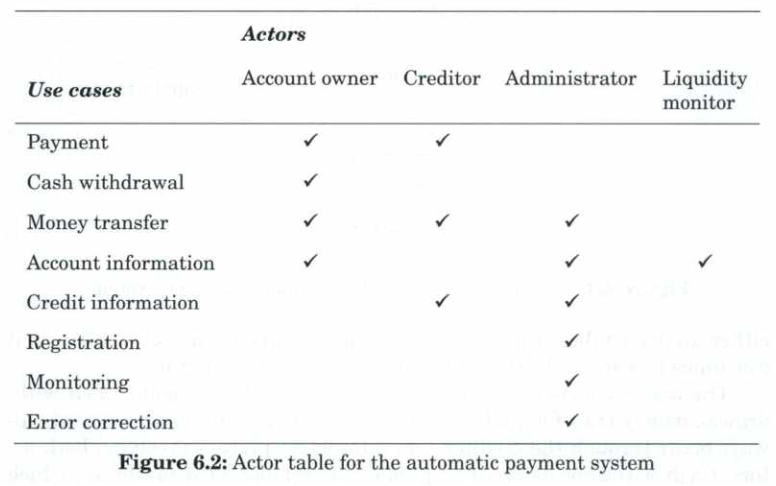
\includegraphics[width=\linewidth*3/4]{parts/3_application_domain_analysis/1_usage/figures/use_cases.png}
\end{figure}

\begin{figure}[H]
    \centering
    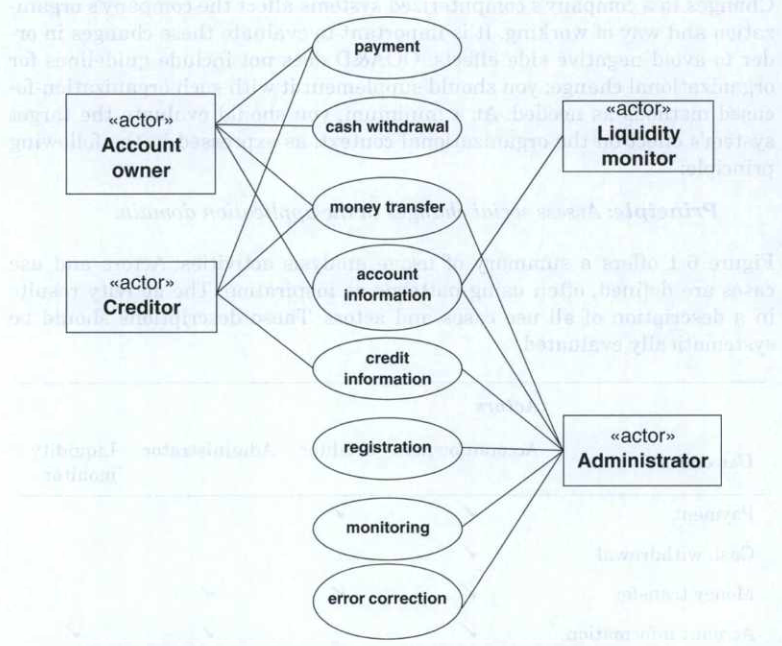
\includegraphics[width=\linewidth*3/4]{parts/3_application_domain_analysis/1_usage/figures/use_cases_diagram.png}
\end{figure}

\section{Find Actors and Use Cases}
Criterion for determening different actors is a dissimilarity of roles. If multiple roles appear the same to the system, they should be consolidated.
\subsection*{Describe actors}
\begin{figure}
    \begin{tabular}{p{\textwidth }}
        \\\hline
        \begin{center}
            Account owner
        \end{center}
        \\\hline
        \begin{description}
            \item[Goal:] person who owns an account. The account owner’s basic need is to make payments with their plastic card.
            \item[Characteristics:] The system’s users include many account owners, with different levels of experience and sophistication.
            \item[Examples:] Account Owner A feels insecure about using a plastic card as a form of payment. Owner A originally got a card be cause it was the only way he could get an ID card for his checks. Owner A only withdraws money from the ATM in emergency situations.
            \item[] Account Owner B is technologically curious and she uses the system often, optimally, and to the limit of its abilities. B has never had major problems in understanding the system’s possibilities, and also examines possibilities that are not obviously accessible.
        \end{description}
        \\\hline
    \end{tabular}
\end{figure}
\subsection*{Describe Use Cases}
Can be described with statechart diagram for a good overview or a use-case specification for more details. It should make use of abstraction, the goal is to collect many possible ways of using the traget system in a few well-chosen use cases.
\chapter{Functions \ooad[139]}
\begin{figure}[H]
    \begin{tabular}{|l|p{12cm}|}
        \hline
        \textbf{Purpose} & \begin{itemize}
            \item To determine the system's information processing capabilitites.
        \end{itemize} \\\hline
        \textbf{Concepts} & \begin{itemize}
            \item Function: A facility for making a model useful for actors.
        \end{itemize} \\\hline
        \textbf{Principles} & \begin{itemize}
            \item Udentify all functions.
            \item Specify only complex funtions.
            \item Check consistency with use cases and the model.
        \end{itemize} \\\hline
        \textbf{Result} & \begin{itemize}
            \item A complete list of functions with specification of complex functions.
        \end{itemize} \\\hline
    \end{tabular}
\end{figure}
Functions focus on what the system can do to assist actors in their work.
When determining requirement for functions:
\begin{itemize}
    \item What is the system going to do?
\end{itemize}
\section{System Functions\ooad[139]}
\begin{figure}[H]
    \textit{\textbf{Function -} A facility for making a model useful for actors.}
\end{figure}
From an analytical perspective a function represents the intent of a system. A function is activated, executed and provides a result. The execution can change the state of a model's components or create a reaction in application or problem domain.
\subsection*{Function Types\ooad[140]}
\begin{description}
    \item[Update] functions are activated by a problem-domain event and result in a change in the model’s state.
    \item[Signal] functions are activated by a change in the m odel’s state and result in a reaction in the context; this reaction might be a display to the actors in the application domain, or a direct intervention in the problem domain.
    \item[Read] functions are activated by a need for information in an actor’s work task and result in the system displaying relevant parts of the model.
    \item[Compute] functions are activated by a need for information in an actor’s work task and consist o f a computation involving information provided by the actor or the model; the result is a display of the computation’s result.     
\end{description}
Functions are not always pure and can be mixture of the above.

\subsection*{Analysing Functions\ooad[143]}
\principle[Identify all functions.]
\principle[Specify only complex functions.]
\principle[Check consistency with use cases and the model.]

\section{Find Functions}
There are two essential aspects when finding functions:
\begin{itemize}
    \item Consider the sources for identifying functions. Where do the systems' function requirements come from.
    \item Consider the level of detail. How detailed should the description of a function be. How specific or general should defining individual functions be?
\end{itemize}
The sources are problem-domain description expressed by it's classes and events. Also the application domain expressed by its use cases.

\begin{itemize}
    \item Classes typically gives read and update functions.
    \item Events typically gives update functions.
    \item Use cases gives all functions.
\end{itemize}
Functions must be described enough for both and overview of total functionality, but also a basis for an agreement between developer and users.\\\\
The result should be a list functional requirements for the system.

\section{Principles}
\begin{description}
    \item[\textit{Identify all functions.}] One of the main purposes of the analysis is to determine the level of ambition for the target system. The complete list of functions is an important element in achieving this.
    \item[\textit{Specify only complex functions.}] We recommend that you describe the functions briefly and informally in a list. However, it may sometimes be necessary to specify certain functions in detail in order to understand them and assess their complexity.
    \item[\textit{Check consistency with use cases and the model.}] The list of functions must be consistent with the list of use cases and the m odel’s classes and events. Checking this can reveal insufficient analysis.
\end{description}